\documentclass[a4paper,10pt]{article}
\usepackage[utf8]{inputenc}
\usepackage{tikz}
\usepackage{latexsym}
\usepackage{amsmath}
\usepackage{amssymb}
\usepackage{amsthm}
\usepackage{tabulary}
\usepackage{algorithm}%%psedocodigo
\usepackage{algorithmic}
%\input{spanishAlgorithmic} % mi archivo de traducción
\usepackage{graphicx}



%opening
\title{Colas con priopidad (Heap's)}
\author{ \Large Luigy Alex Machaca Arcana \\Luigy.mach.arc@gmail.com \\ Universidad Nacional de San Agustín \\ Escuela Profesional de Ciencia de la Computación \\ Análisis y Estructura de Datos }

\begin{document}
\maketitle
\begin{abstract}
Los  heaps son estructuras frecuentemente usadas para implementar colas de prioridad, en dicha estructura la extracción de datos es mas óptima que otras estructuras, sea el mínimo o máximo según sea el caso. Existen diferentes formas de implementar este tipo de estructuras, algunas de ellas son binary heap, binomial heap, fibonacci heap. En este artículo se analiza el como se implementa y algunas operaciones con estas estructuras.
\end{abstract}

\section{Introducción}

Muchas veces necesitamos usar estructuras parcialmente ordenadas para recurrir al o a los elementos con mayor prioridad. 

Por ejemplo para el algoritmo de Kruskal y Prim para el cálculo del
árbol de expansión mínimo de un grafo etiquetado, ó para el algoritmo de Dijkstra para el cálculo de caminos
mínimos en un grafo etiquetado, por lo que las aristas deben estar almacenadas en una estructura parcialmente ordenada. Otro caso se da cuando queremos rankear los elementos, de tal forma que
podemos obtener un top 5, top 10, etc. ya que solo nos importan los primeros elementos. Así como estas aplicaciones, existen muchas otras que necesitan de estructuras parcialmente ordenadas. Entre este tipo de estructuras se encuentran las \textit{priority queues} \footnote{\textbf{Una cola de prioridades} es una estructura de datos en la que los elementos se atienden en el orden indicado por una prioridad asociada a cada uno}, tales como listas enlazadas, binary heaps, binomial heaps, fibonacci heaps,\cite{diapos} Las estructuras a analizar en este artículo son: Binary Heap, la cuales estan basadas en un árbol binario; y Binomial Heap, que está basada en un árbol binomial. Además existe un método de ordenación llamado Heapsort, que utiliza funciones del binary heap. El costo de este algoritmo es (n log n).




\section{Conceptos previos}
\subsection{Priority queue}
Priority Queue es una estructura de datos fundamental que permite el acceso solo al elemento mínimo o máximo \footnote{orden \textbf{ascendente}  para extraer el maximo, o en su defecto \textbf{descendente} para extraer el mínimo} \cite{cormen}
Una implementación de las priority queue es el Heap. Estas deben soportar por lo menos las siguientes operaciones: Insertar, Encontrar menor o mayor, Eliminar menor o mayor. 


\subsection{Heaps}
Un Heap es una estructura de datos especializada basada en el concepto de árbol (\textit{se utilizan para el ordenamiento de datos \textit{HeapSort} y para implementar colas de propiedades} ), estas satisface la siguiente propiedad: Para todo nodo A cuyo padre es P, A debe estar ordenado respecto a P. Entre algunos tipos de Heap estan\cite{diapos}: Binary
Heap, Binomial Heap, Fibonacci Heap, Radix Heap, d-ary Heap, Soft Heap, etc. El Min-Max Heap es un caso especial, ya que deja de ser un árbol.



\subsection{Binary Heap}
Un binary heaps es un caso particular y bastante sencillo, dicha estructura esta basada en un árbol  binario parcialmente ordenado, que puede verse como un árbol binario con dos propiedades(Restricciones) adicionales\cite{AEDc++} :
\begin{itemize}
	\item Cada nodo tiene un valor mayor o menor 		(orden ascendente u orden descendente) que cualquiera de sus hijos.
	\item Este árbol binario tiene que tiene que ser completo, es decir debe tener todos sus nodos, con
excepción de que tal ves no existan todos los nodos en el último nivel.	
\end{itemize}
Cumpliendo estas anteriores propiedades el Binary Heap se puede representar a través de un vector como se muestra en la Figura \ref{fig:heapMax}.
A partir de esto se puede deducir que:
\begin{itemize}
	\item Para cada elemento en la posicion i \footnote{como \textbf{i} es la poscion siempre sera un entero.}  .
	\item Sus hijo deben de estar(dentro del array), en las posiciones \textbf{2k} y \textbf{2k+1}, siendo el primero para hijo izquierdo y el segundo para el derecho respectivamente.
	\item para encontrar el padre de k solo se debe realizar una división entera del índice k/2.
\end{itemize}


\begin{figure}[!ht]
	\caption{Max Heap, representado a través de un array}
	\label{fig:heapMax} 
	\begin{center}
	  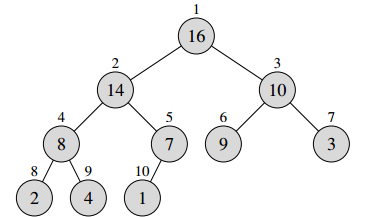
\includegraphics[scale=0.6]{heap_maximo.jpg}	
	 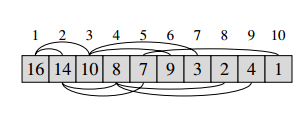
\includegraphics[width=0.6\textwidth]{heap_array.jpg}
	\end{center}	
\end{figure}


Para el binomial heap una de las operaciones más importantes es \textbf{Heapify}, que
se encarga de hacer que se cumpla la propiedad de los Heaps En el Algoritmo (\ref{Heapify}) se expone el pseudocódigo.


\begin{algorithm}[1]

	\REQUIRE data(vector de dato), i( posición del nodo a calcular), cmp(Funcion comparacion)
	\caption{Heapity} \label{alg:algoritmoHeapify}
\end{algorithm}






\section{asas}




\newpage
	\begin{thebibliography}{9}

\bibitem[1]{cormen}
Thomas H. Cormen, Charles E. Leiserson, Ronald L. Rivest, Cliford Stein.
\textit{Introduction to Algorithms}. The MIT Press, Cambridge, Massachusetts, 3rd
Edition, 2009.

\bibitem[2]{diapos}
Kevin Wayne,\textit{ Binary and Binomial Heaps - Theory of Algorithms}. Princeton
University, 2002.

\bibitem[3]{AEDc++}
Antonio Garrido Carrillo y Joaquin Valdivia , Antonio Garrido Carrillo, Joaquín Fernández Valdivia
\textit{Abstracción y Estructuras de datos en C++}
Delta Publicaciones, 2006 .

\bibitem[4]{priorityQueue}  
Alonso Ramirez Manzanares \textit{Colas de prioridad ( priority queues)} - Computación y Algoritmos, 2012.   
  
  
	\end{thebibliography}
	
	
	
\end{document}



